\documentclass[paper=a4, parskip=half]{scrreprt}

\usepackage{etex}
\usepackage[utf8]{inputenc}
\usepackage[T1]{fontenc}

\usepackage{lmodern}
\usepackage[ngerman]{babel}

\usepackage{bibgerm} 
\usepackage{cite}
\usepackage{url}

\usepackage{graphics}

\usepackage[hypertexnames=false, linktocpage]{hyperref}

\usepackage{titling}
\usepackage{graphicx}
\graphicspath{ {./Bilder/} }
\usepackage{wrapfig}
\usepackage{float}
\usepackage{adjustbox}
\usepackage{setspace}
\usepackage{hyperref}
\usepackage[acronym]{glossaries}
\usepackage[printonlyused]{acronym}
\usepackage{datetime}
\usepackage[normalem]{ulem}

\usepackage{subfiles} % Best loaded last in the preamble

\subfile{Meta/glossary}

\setcounter{tocdepth}{1}

%Custom commands
\newcommand{\Genderly}{\textsc{Genderly}}


\begin{document}
%TC:ignore
\title{Software Requirements Specification} % Meta

\subfile{Meta/coversheet}
\subfile{Meta/guides}
%\subfile{Meta/glossary}

%TC:endignore
\chapter{Einführung}

\section{Zweck}
Die \ac{SRS} beschreibt die funktionalen und nicht-funktionalen Anforderungen für den prototypischen Software-Release der Anwendung \Genderly{}. Das Dokument wurde für die Nutzung durch die Teammitglieder des Projekts angefertigt. Sie implementieren und verifizieren die korrekte System-Funktionalität.\\
Wenn nicht anders angegeben, gelten alle hier aufgeführten Anforderungen für  den prototypischen Software-Release 1.0.0.

\section{Dokumentkonventionen}
Für das Dokument finden keine speziellen typografischen Konventionen Verwendung.

\section{Projekt-Scope und Produkt-Features}
\Genderly{} wird Student*innen, Schüler*innen und anderen Textverfasser*innen eine Möglichkeit zur Texterfassung, -analyse und Generierung eines genderneutralen Vorschlagstexts bieten, basierend auf einem eingegebenen Text. Eine hierzu angefertigte, detaillierte Beschreibung ist im Vision and Scope Dokument für \Genderly{} zu finden. Ebenso sind dort die Features einsehbar, die in dieser Version ganz oder teilweise implementiert werden sollen.

\section{Referenzen}
\begin{table}[hbt!]
\begin{tabular}{ll}
\textbf{1.} & Witteborn-Demir, Gökhan; Jacobsen, Jan Felix; Podkolsin, Dennis;\\
   &Koppelmann, Marcus. \Genderly{} Vision and Scope Document
\end{tabular}
\end{table}


\chapter{Projektbeschreibung}
\section{Produkt-Perspektive}
\Genderly{} ist eine neue Softwareapplikation, welche das Konzept eines Übersetzungsprogramms und der Listen für genderneutrale Wörter miteinander vereint. \Genderly{} ist eine Webanwendung, die für sich steht und keine externen Schnittstellen zu anderen Softwaresystemen besitzt.

\pagebreak

\section{Benutzerklassen und Charakteristiken}

\begin{table}[!htb]
\begin{tabular}{ll}
\textbf{Student*innen} & Da im akademischen Raum das Gendern deutlich und \\ 
(Hauptzielgruppe) & umfassend an Bedeutung gewinnt, wird es sich bei den \\
& Nutzer*innen sehr wahrscheinlich zu einem großen Anteil\\ 
& um Student*innen handeln. Deswegen orientiert sich die \\
& Anwendung besonders an dieser speziellen Zielgruppe. Die \\
& Anwendung hilft den Student*innen beim einfachen und \\
& korrekten Gendern in wissenschaftlichen Texten. \vspace{0.15cm} \\

\textbf{Dozent*innen} & Auch in diesem Fall ist die Findung der Benutzergruppe \\
& mit der zunehmenden Bedeutung im akademischen Raum \\
& zu begründen. Der Einsatz der Anwendung findet hier vor- \\
& wiegend im didaktischen und pädagogischen Zusammenhang \\
& statt. Die Dozent*innen verfolgen dabei das Ziel ihren Lehr- \\
& auftrag zu erfüllen, welcher auch die Vermittlung der Gleich- \\
& berechtigung der Geschlechter beinhaltet. \vspace{0.15cm} \\

\textbf{Lehrkräfte \&} & Die Lehrkräfte haben ein besonders hohes Interesse an der \\
\textbf{Schüler*innen} & einfachen und flexiblen Anwendung des Produkts. Sie ver- \\
& folgen dabei das Ziel ihren Lehrauftrag zu erfüllen, welcher \\
& auch die Vermittlung der Gleichberechtigung der Geschlechter \\
& beinhaltet. Schüler*innen möchten gleichzeitig sehr leicht \\
& lernen. Beide nutzen die Software als Hilfsmittel während des \\
& Schreibens. Besonders hervorzuheben ist hierbei das potenzielle \\
& Alter der Anwender*innen sowohl in das eine, als auch in das \\
& andere Extrem. \vspace{0.15cm} \\

\textbf{Politiker*innen} & In Teilen der Politik wird vermehrt Wert auf inklusives \\
& Schreiben gelegt. Das Ziel dabei ist es, dass sich dass Publikum \\
& besser angesprochen und stärker einbezogen fühlt, damit die \\
& Politiker*innen eine möglichst große Wählerschaft erreichen. \vspace{0.15cm} \\

\textbf{Journalist*innen} & In Teilen des Journalismus wird vermehrt Wert auf inklusives \\
& Schreiben gelegt. Das Ziel dabei ist es, dass sich mehr \\
& Leser*innen einbezogen und angesprochen fühlen, damit die \\
& Journalist*innen eine möglichst große Leserschaft erreichen. \vspace{0.15cm} \\
\end{tabular}
\end{table}

\pagebreak

\section{Ausführungsumgebung}
\begin{table}[!htb]
\begin{tabular}{ll}
\textbf{AU-1} & \Genderly{} muss mithilfe der folgenden Webbrowsern erreichbar sein: \\
& Google Chrome (alle aktuellen Versionen); Firefox (alle aktuellen Versionen);\\
& Microsoft Edge (alle aktuellen Versionen); Safari (alle aktuellen Versionen) \vspace{0.15cm} \\
\textbf{AU-2} & Der serverseitige Betrieb der Anwendung muss auf MacOS, Windows \\
& oder Linux möglich sein, wobei eine vorherige Installation von Java 8 \\
& zwingend notwendig ist. \vspace{0.15cm}\\
\textbf{AU-2} & \Genderly{} muss den Zugriff von allen internetfähigen Geräten, welche \\
& von den festgestellten Benutzerklassen genutzt werden, erlauben, \\
& unabhängig von dem Ort an dem sich das Endgerät befindet. \vspace{0.15cm}\\
\end{tabular}
\end{table}

\section{Einschränkungen in Design und Implementation}
\begin{table}[!htb]
\begin{tabular}{ll}
\textbf{Anforderung 1} & Die Anforderungsdokumentation muss den gelehrten Dokumentations- \\
& konventionen entsprechen, die wir in den Vorlesungen ausführlich \\ 
& durchgenommen haben. \vspace{0.15cm} \\

\textbf{Anforderung 3} & Das Frontend muss mit HTML5, CSS3, JavaScript und \\
& Thymeleaf verfasst sein. \vspace{0.15cm}\\
\textbf{Anforderung 3} & Der Code für das Backend, welches mit dem Frontend und einer \\
& Datenbank kommuniziert, muss mit Java unter Verwednung von \\
& Spring und Maven erstellt werden. \vspace{0.15cm}\\
\textbf{Anforderung 2} & Die Datenbank muss als \ac{DBMS} \\
& SQLite verwenden. \vspace{0.15cm}\\
\textbf{Anforderung 4} & Die Arbeit der Entwickler muss auf dem GitHub Repository der \\
& Organisation stattfinden. \vspace{0.15cm}\\
\end{tabular}
\end{table}

\pagebreak

\section{Annahmen und Abhängigkeiten}
\begin{table}[!htb]
\begin{tabular}{ll}
\textbf{Annahme 1} & Nutzer*innen haben Zugang zu einem internetfähigen Gerät. \vspace{0.15cm} \\
\textbf{Annahme 2} & Die Web-App wird auf einem dem Anfragevolumen gerecht \\
& werdenden System betrieben. \vspace{0.15cm} \\
\end{tabular}
\end{table}

\begin{table}[!htb]
\begin{tabular}{ll}
\textbf{Abhängigkeit 1} & Benutzer*innen verfügen über einen Internetzugang. \vspace{0.15cm} \\
\textbf{Abhängigkeit 2} & Wenn Benutzer*innen internetfähige Geräte, wie z.B. \\
& Smartboards oder Tablets nutzen, muss \Genderly{}\\
& mit diesen Geräten kompatibel sein. \vspace{0.15cm}\\
\textbf{Abhängigkeit 3} & Der genderneutrale Sprachstil sollte sich nicht ändern. \vspace{0.15cm}\\
\end{tabular}
\end{table}


\chapter{System Features}
% end me :c
\section{Web Access}
\subsection{Beschreibung}
Die Anwendung ist über eine eigene Weboberfläche aufrufbar. Priorität = Hoch
\subsection{Funktionale Anforderungen}
\begin{table}[!htb]
\begin{tabular}{ll}
\textbf{Anforderung 1} & Wenn Nutzer*innen die Webanwendung über einem Web- \\
& browser und mit einer stabilen Internetverbindung aufrufen, \\
& muss das System ein Bedienfeld für die Verwendung der \\
& nachfolgenden System Features bereitstellen. Das Layout des \\
& Bedienfelds wird in Kapitel \ref{Benutzerschnittstellen} (Benutzerschnittstellen) \\
& genauer definiert. \vspace{0.15cm} \\

\end{tabular}
\end{table}

\section{Texteingabe}
\subsection{Beschreibung}
Der zu gendernde Text der Nutzer*innen wird über ein eigenes dafür vorgesehenes Eingabefeld aufgenommen. Priorität = Hoch
\subsection{Funktionale Anforderungen}
\begin{table}[!htb]
\begin{tabular}{ll}
\textbf{Anforderung 1} & Nach erfolgreichen Aufruf der Anwendung, muss \Genderly{} \\
& den Nutzer*innen die Möglichkeit bieten den Eingabetext in ein \\
& Textfeld einzugeben. \vspace{0.15cm} \\
\end{tabular}
\end{table}

\section{Substantiv-Analyse}
\subsection{Beschreibung}
Genderbare Substantive werden ermittelt und ggf. ausgetauscht. Priorität = Hoch
\subsection{Funktionale Anforderungen}
\begin{table}[!htb]
\begin{tabular}{ll}
\textbf{Anforderung 1} & Nach Eingabe des Texts und Betätigung des „Gendern“ Buttons, \\
& muss \Genderly{} die Textanalyse starten. \vspace{0.15cm} \\
\textbf{Anforderung 2} & Wenn der Eingabetext leer ist, muss \Genderly{} den Vorgang \\
& abbrechen und auf eine erneute Eingabe und Betätigung der \\
& Nutzer*innen warten. \vspace{0.15cm} \\
\textbf{Anforderung 3} & Wenn der Eingabetext nicht leer ist, muss \Genderly{} den Eingabe- \\
& text in eine Menge von einzelnen Wörtern zerlegen und in dieser \\
& Wortmenge nach Substantiven suchen. \vspace{0.15cm} \\
\textbf{Anforderung 4} & Wenn in der Wortmenge kein Substantiv gefunden wurde, muss \\
& die Anwendung den Vorgang abbrechen und auf eine erneute \\
& Eingabe und Betätigung der Nutzer*innen warten. \vspace{0.15cm} \\
\textbf{Anforderung 5} & Wenn in der Wortmenge Substantive gefunden wurden, muss \\
& \Genderly{} diese Wörter mit den Einträgen in der Datenbank \\
& abgleichen. \vspace{0.15cm} \\
\textbf{Anforderung 5} & Wenn genderneutrale Ersatzworte gefunden wurden, muss die \\
& Applikation die entsprechenden Substantive in dem Text mit \\
& den Ersatzworten austauschen. \vspace{0.15cm} \\
\end{tabular}
\end{table}

\pagebreak

\section{Artikel-Analyse}
\subsection{Beschreibung}
Durch Gendering verfälschte Artikelzuordnungen werden ermittelt und ggf. ausgetauscht. Priorität = Hoch
\subsection{Funktionale Anforderungen}
\begin{table}[!htb]
\begin{tabular}{ll}
\textbf{Anforderung 1} & Während der Substantiv-Analyse, muss \Genderly{} prüfen, ob \\
& durch den Austausch der Substantive sich die zugehörigen \\
& Artikel geändert haben. \vspace{0.15cm} \\
\textbf{Anforderung 2} & Wenn sich der zugehörige Artikel verändert hat, muss \Genderly{} \\
& den nun verfälschten Artikel mit dem passenden austauschen. \vspace{0.15cm} \\
\end{tabular}
\end{table}

\section{Textausgabe}
\subsection{Beschreibung}
Der genderneutrale Ausgabetext wird visualisiert, sodass Nutzer*innen den Ausgabetext noch nachbearbeiten können. Priorität = Hoch
\subsection{Funktionale Anforderungen}
\begin{table}[!htb]
\begin{tabular}{ll}
\textbf{Anforderung 1} & Nach erfolgreichen Austausch der genderbaren Wörter, muss \\
& \Genderly{} den Nutzer*innen die Möglichkeit bieten den gender- \\
& neutralen Text in einem Textfeld nachzubearbeiten und aus dem \\
& Textfeld zu kopieren. \vspace{0.15cm} \\
\end{tabular}
\end{table}

\pagebreak

\section{Sprachauswahl}
\subsection{Beschreibung}
Die Sprache des Eingabe- und Ausgabetextes ist auswählbar. Priorität = Mittel
\subsection{Funktionale Anforderungen}
\begin{table}[!htb]
\begin{tabular}{ll}
\textbf{Anforderung 1} & Nach erfolgreichem Aufruf der Anwendung sollte \Genderly{} \\
& den Nutzer*innen die Möglichkeit bieten die Sprache des Ein- \\
& und Ausgabetextes auszuwählen. \vspace{0.15cm} \\
\end{tabular}
\end{table}

\section{Gendering-Stilauswahl}
\subsection{Beschreibung}
Der Gendering-Stil des durch eine Analyse auszugebenden Text-Vorschlags ist auswählbar. Priorität = Mittel
\subsection{Funktionale Anforderungen}
\begin{table}[!htb]
\begin{tabular}{ll}
\textbf{Anforderung 1} & Nach erfolgreichem Aufruf der Anwendung sollte \Genderly{} \\
& den Nutzer*innen die Möglichkeit bieten den Gendering-Stil \\
& des Ausgabetexts auszuwählen. \vspace{0.15cm} \\
\end{tabular}
\end{table}

\pagebreak

\section{Theme-Anpassung}
\subsection{Beschreibung}
Die farbliche Darstellung der Anwendung kann durch Nutzer*innen angepasst werden. Priorität = Mittel
\subsection{Funktionale Anforderungen}
\begin{table}[!htb]
\begin{tabular}{ll}
\textbf{Anforderung 1} & Nach erfolgreichem Aufruf der Anwendung sollte \Genderly{} \\
& den Nutzer*innen die Möglichkeit bieten die farbliche \\
& Darstellung der Anwendung festzulegen. \vspace{0.15cm} \\
\end{tabular}
\end{table}

\chapter{Datenanforderungen}
\section{Logisches Datenmodell}
\begin{figure}[hbt!]
  \centering
  \fbox{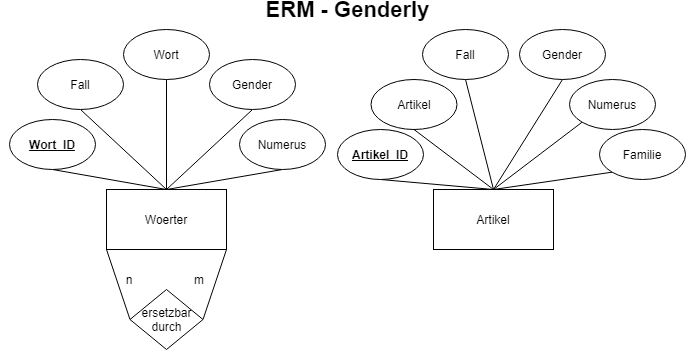
\includegraphics[scale=1.0]{Bilder/ERM.png}}
  \vspace{-0.25cm}
  \caption[ERM der Datenbank]{ERM der Datenbank}
  \label{fig:Bahn-RBC}
\end{figure}

\pagebreak

\section{Datenkatalog}
\begin{figure}[hbt!]
  \centering
  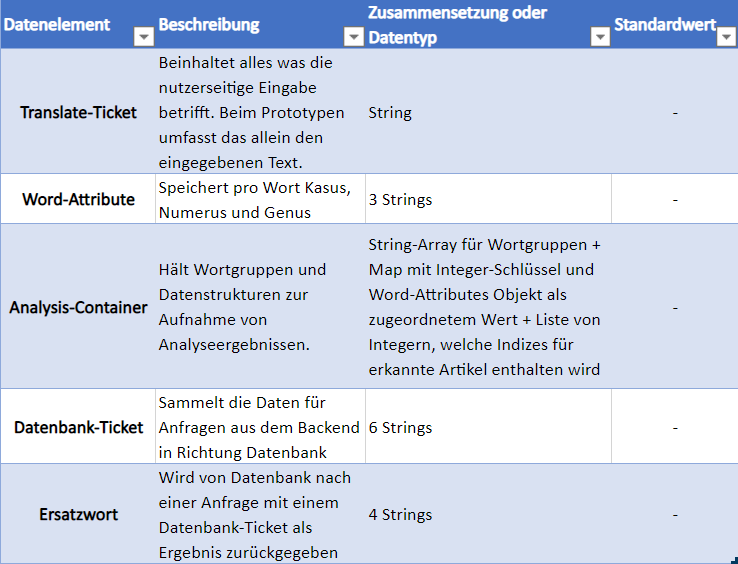
\includegraphics[scale=1.0]{Bilder/Datenkatalog.png}
  \vspace{-0.25cm}
\end{figure}

\section{Reports}
Zwecks Datenschutz werden keine Reports zu durchgeführten Analysen erhoben.

\pagebreak

\section{Datenbeschaffung, Integritätsprüfung, Speicherung und Datenentledigung}
\begin{table}[!htb]
\begin{tabular}{ll}
\textbf{Anforderung 1} & Die Wortlisten für die Substantive und Artikel müssen \\
& basierend auf den Bedürfnissen der Benutzerklassen erhoben \\
& werden und auf diese zugeschnitten sein. \vspace{0.15cm} \\
\textbf{Anforderung 2} & Nach Abschluss einer Nutzer*innenanfrage muss die \\
& Anwendung die Benutzereingaben löschen. \vspace{0.15cm} \\
\textbf{Anforderung 2} & Die Datensätze innerhalb der Datenbank müssen alleine \\
& vom Serverbetreiber bearbeitet und entfernt werden können. \vspace{0.15cm} \\
\end{tabular}
\end{table}


\chapter{Anforderungen an externe Schnittstellen}
\section{Benutzerschnittstellen} \label{Benutzerschnittstellen}
\begin{table}[!htb]
\begin{tabular}{ll}
\textbf{BS-1} & Aufgrund der Vielfältigkeit der Benutzerklassen muss \Genderly{} eine \\
& intuitive Oberfläche haben. \vspace{0.15cm} \\
\textbf{BS-2} & Das Layout von \Genderly{} sollte sich grundlegend an dem Design eines \\
& Übersetzungsprogramms orientieren. \Genderly{} muss den Nutzer*innen \\
& die Möglichkeit bieten, den Eingabetext in einem Textfeld eingeben zu \\
& können und die Analyse des eingegebenen Texts und die Generierung des \\
& genderneutralen Alternativtexts mit einem Knopf zu starten. Außerdem \\
& muss \Genderly{} ein weiteres Textfeld für die Textausgabe und Nach- \\
& bearbeitung des Ausgabetextes bieten. \\
& (siehe Abbildung \ref{fig:Screenshot}) \vspace{0.15cm} \\
\textbf{BS-3} & Die Anwendung sollte ein Auswahlmenü für die Sprachauswahl, den \\
& Gendering-Stil und die Theme-Auswahl bereitstellen. \vspace{0.15cm}\\ 
\textbf{BS-3} & Auf der Webseite sollte ein Link zum GitHub Repository von \Genderly{} \\
& vorhanden sein. \vspace{0.15cm}\\
\end{tabular}
\end{table}

\begin{figure}[hbt!]
  \centering
  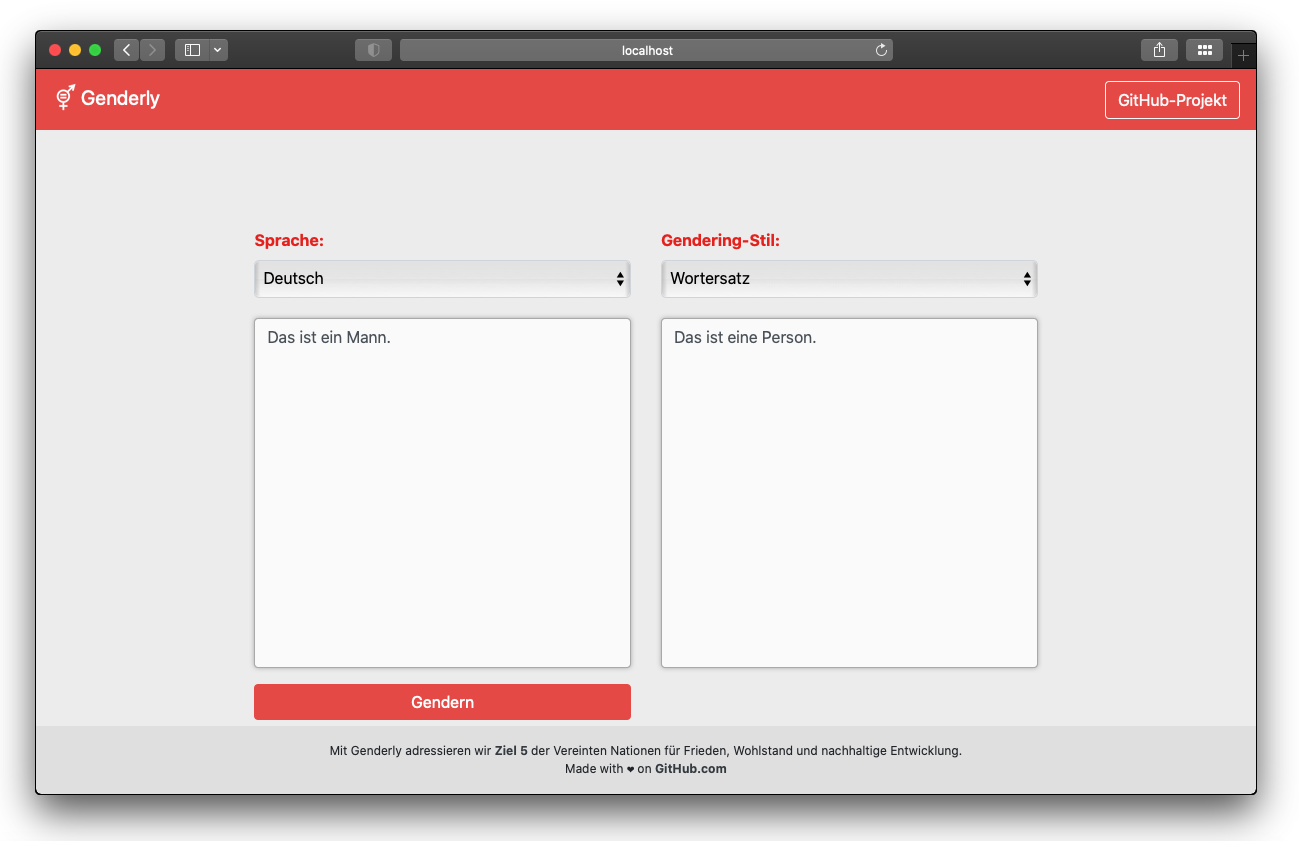
\includegraphics[scale=0.45]{Bilder/Screenshot.PNG}
  \vspace{-0.25cm}
  \caption[Screenshot der Webanwendung]{Screenshot der Webanwendung}
  \label{fig:Screenshot}
\end{figure} 

\section{Softwareschnittstellen}
Es wurden keine Softwareschnittstellen identifiziert.

\section{Hardwareschnittstellen}
Es wurden keine Hardwareschnittstellen identifiziert.

\section{Kommunikationsschnittstellen}
Es wurden keine Kommunikationsschnittstellen identifiziert.

\chapter{Qualitätsmerkmale}
\section{Benutzbarkeit}
Die Benutzbarkeit ist bei \Genderly{} aufgrund der breiten Spanne an verschiedenen Nutzer*innen besonders wichtig.
Die einfache Handhabung der Weboberfläche steht an erster Stelle und ist ein großer Bestandteil des Designkonzepts.
\begin{table}[!htb]
\begin{tabular}{ll}
\textbf{Anforderung 1} & Das Layout von \Genderly{} muss sich an dem Design eines \\
& Übersetzungsprogramms orientieren. Dadurch besitzt die \\
& Anwendung eine intuitive Bedienoberfläche und verfügt darüber \\
& hinaus auch über einen Wiedererkennungscharakter. \vspace{0.15cm}\\ 
\textbf{Anforderung 2} & \Genderly{} muss den Nutzer*innen die Möglichkeit bieten die \\
& Textanalyse und Generierung eines genderneutralen Texts mit \\
& einem einzigen Knopfdruck zu starten. \vspace{0.15cm}\\ 
\textbf{Anforderung 3} & \Genderly{} muss mit einem Webbrowser und einer Internet- \\
& verbindung von jedem mobilen Endgerät aus aufrufbar sein. \vspace{0.15cm}\\ 
\textbf{Anforderung 4} & Mit Hilfe \Genderly{}s müssen 90\% der Erstnutzer*innen in \\
& der Lage sein in kürzester Zeit aus ihrem Eingabetext \\
& problemlos einen genderneutralen Text zu generieren. \vspace{0.15cm}\\
\textbf{Anforderung 5} & Die Weboberfläche sollte aus wenig Elementen bestehen. Dies \\
& erhöht die Übersichtlichkeit der Anwendung. \vspace{0.15cm}\\
\end{tabular}
\end{table}

\section{Performance}
\begin{table}[!htb]
\begin{tabular}{ll}
\textbf{Anforderung 1} & Bei Aufruf durch die Nutzer*innen sollte die Webanwendung \\
& innerhalb von 5 Sekunden verfügbar sein. \vspace{0.15cm}\\ 
\textbf{Anforderung 2} & Nach Eingabe eines Texts und Start der Analyse, sollte \Genderly{} \\
& den Ausgabetext innerhalb von maximal 30 Sekunden generieren. \vspace{0.15cm}\\ 
\end{tabular}
\end{table}

\section{IT-Sicherheit}
Das Thema IT-Sicherheit nehmen wir sehr ernst. Aufgrund dessen haben wir bereits zu Beginn eine Security Policy eingeführt welche öffentlich in dem GitHub Repository einsehbar ist. 
\begin{table}[!htb]
\begin{tabular}{ll}
\textbf{Anforderung 1} & Die Anwendungsarchitektur muss Datenströme sorgfältig vor \\
& der Außenwelt schützen. \vspace{0.15cm}\\ 
\end{tabular}
\end{table}

\section{Datensicherheit}
\begin{table}[!htb]
\begin{tabular}{ll}
\textbf{Anforderung 1} & \Genderly{} muss SQL-Injektion-Attacken erkennen und \\
& verhindern können. \vspace{0.15cm}\\ 
\textbf{Anforderung 2} & Die Datenbank muss vor Zugriffen und unbefugter \\
& Manipulation geschützt sein. \vspace{0.15cm}\\ 
\end{tabular}
\end{table}

\section{Verfügbarkeit}
\begin{table}[!htb]
\begin{tabular}{ll}
\textbf{Anforderung 1} & \Genderly{} sollte nach offizieller Inbetriebnahme zu 95\% der Zeit verfügbar sein. \\
& Ausnahme davon sind geplante Zeiten für Wartungsarbeiten. \vspace{0.15cm}\\ 
\end{tabular}
\end{table}


\chapter{Anforderungen zu Internationalisierung und Verortung}
\Genderly{} hat das Ziel in erster Form in deutscher Sprache zu funktionieren. In Zukunft ist der Ausbau und die Bereitstellung verschiedener Sprachen angedacht um eine größere Zielgruppe zu erreichen. \\
Somit sollte \Genderly{} in Zukunft Texte auch in anderen Sprachen und anderen Gendering-Stilen gendern können.



%TC:ignore

%Glossar
\printglossary
\pagebreak

%\nocite{*}
%\bibliography{Literatur}
%\bibliographystyle{alphadin}


%\subfile{Anhang/main}
%TC:endignore

\end{document}